\documentclass[12pt,letterpaper]{article}
\usepackage{fullpage}
\usepackage[top=2cm, bottom=4.5cm, left=2.5cm, right=2.5cm]{geometry}
\usepackage{amsmath,amsthm,amsfonts,amssymb,amscd}
\usepackage{lastpage}
\usepackage{enumerate}
\usepackage{fancyhdr}
\usepackage{mathrsfs}
\usepackage{xcolor}
\usepackage{graphicx}
\usepackage{listings}
\usepackage{hyperref}
\usepackage{amsmath}
\usepackage{mathtools}
\usepackage{tikz}
\usepackage{array}
\usetikzlibrary{matrix}

\hypersetup{%
  colorlinks=true,
  linkcolor=blue,
  linkbordercolor={0 0 1}
}
 
\renewcommand\lstlistingname{Section}
\renewcommand\lstlistlistingname{Algorithms}
\def\lstlistingautorefname{Alg.}

\lstdefinestyle{Python}{
    language        = Python,
    frame           = lines, 
    basicstyle      = \footnotesize,
    keywordstyle    = \color{blue},
    stringstyle     = \color{green},
    commentstyle    = \color{red}\ttfamily
}

\setlength{\parindent}{0.0in}
\setlength{\parskip}{0.05in}

% Edit these as appropriate
\newcommand\course{CSE 3500}
\newcommand\hwnumber{0}                  % <-- homework number
\newcommand\NetIDa{rjf23002}           % <-- NetID of person #1
\newcommand\NetIDb{}           % <-- NetID of person #2 (Comment this line out for problem sets)

\pagestyle{fancyplain}
\headheight 35pt
\lhead{\NetIDa}
\lhead{\NetIDa\\\NetIDb}                 % <-- Comment this line out for problem sets (make sure you are person #1)
\chead{\textbf{\Large Homework \hwnumber}}
\rhead{\course \\ \today}
\lfoot{}
\cfoot{}
\rfoot{\small\thepage}
\headsep 1.5em

\begin{document}

\section*{Problem 0}
I have signed the Google Form. I have just attached the response page of the Google Form to the end of this PDF.

\section*{Problem 1}
Hi there! My name is Ryan Cheung and I am a final year/ senior student. 
I'm currently on a fall exchange program here in UConn, and I'm originally from Singapore studying at the National University of Singapore. 
I really enjoy software engineering, and hope to branch out in that field in the future. \\

My favourite programming language would be Python for algo questions, and Java or TypeScript in general. 
I hope to learn more about distributed databases and blockchain in the future, 
and I'm currently taking a blockchain class which I find really interesting.
I currently do a lot of leetcode as I'm hunting for jobs as a senior, 
so what I hope to take away from this class is to learn how to do formal proofs properly, which would aid me in my interview process.

\section*{Problem 2}

\begin{enumerate}
  \item
    n!
  \item
    $\dbinom{n}{3}$
  \item 
    $2^n - 1$
\end{enumerate}

\section*{Problem 3}

\begin{enumerate}
  \item
    \begin{enumerate}[a)]
      \item A = O(B) holds as A is polynomial while B is exponential, where exponential dominates. 
      So A is bounded by B.
      \item A = $\Theta(B)$ holds as we can log both sides, forming  
      $lgn^{lgc}$ and $lgc^{lgn}$ where we bring down the powers to get
      $lgn * lgc$ and $lgc * lgn$.
      \item A = O(B) holds as simplifying A without constants results in 
      n! = $n^{0.5} * n^n * n^{-1}$ where n! = $n^{n - 0.5}$.
      Thus, $n^n$ dominates.
      \item A = $\Omega(B)$ holds. Similar to part a) except the opposite.
    \end{enumerate}
  \item
    (d), (f), (a), (c), (b), (e)
\end{enumerate}

\section*{Problem 4}

\begin{enumerate}
  \item
    The main goal of this problem is that given a string s1, we want to find the longest common subsequence (LCS) in string s2.
    For a character c in s1, it can either be in the LCS or it could not be.
    If we were to do this in a brute force approach, we could solve it recursively, where we have 2 choices: 
    we can check if c is in s2, or take c out and compare the next character in s1 against s2. \\
    This leads to a structure of a decision tree, where at each step we branch out to 2 different decisions. \\
    In a code format, we could define a recursive helper function dfs(i, j) that takes in 2 parameters: i and j being the indexes of the strings s1 and s2.
    At each step, we see if the characters at index i, j are equal or different, which will affect our final costs. Our base cases can then be when either i has reached the end of s1 or j has reached the end of s2. \\
    
    Runtime: $O(2^n)$   \\
    
    Correctness: The brute force solution is recursive in nature, 
    so it enumerates all possible combinations.
    Assuming that our base cases are defined correctly, the smaller subproblems would produce the right results.
    Since our solution is recursive in nature, our bigger problems which build off the smaller ones 
    will therefore have the correct results as well.
  \item 
    Recurrence: Using our defined helper function dfs(i, j), 
    a recurrence relation can be defined as per following for non base cases: \\
    \[
        dfs(i, j)= 
    \begin{dcases}
        dfs(i + 1, j + 1) + 1,& \text{if } str1[i] == str2[j] \\
        max(dfs(i + 1, j), dfs(i, j +1))  & \text{otherwise}
    \end{dcases}
    \]
  \item 
    We can convert this into a DP problem by first memoizing the sub problems with a hashmap/ dictionary.
    To avoid recursion and instead use an iterative approach, we could utilize a 2D grid instead.
    The size of our grid would be (m + 1) * (n + 1), where m = len(s1) and n = len(s2).
    We require m + 1 instead of m to initialize base cases, e.g when str1 is an empty string "", and str2 is of some arbitrary non empty string "ACG...".
  \item 
    Each entry in the table would refer to the LCS that can be formed up to the substrings from indexes s1[0:i] and s2[0:j].
  \item 
            \lstset{caption={DP Diagram}}
            \begin{lstlisting}[style = Python]
                   -  T  C  G  G  A  A  T  A  A
                - [0, 0, 0, 0, 0, 0, 0, 0, 0, 0] 
                A [0, 0, 0, 0, 0, 1, 1, 1, 1, 1] 
                C [0, 0, 1, 1, 1, 1, 1, 1, 1, 1] 
                A [0, 0, 1, 1, 1, 2, 2, 2, 2, 2] 
                G [0, 0, 1, 2, 2, 2, 2, 2, 2, 2] 
                G [0, 0, 1, 2, 3, 3, 3, 3, 3, 3] 
                T [0, 1, 1, 2, 3, 3, 3, 4, 4, 4] 
                T [0, 1, 1, 2, 3, 3, 3, 4, 4, 4] 
                A [0, 1, 1, 2, 3, 4, 4, 4, 5, 5] 
                C [0, 1, 2, 2, 3, 4, 4, 4, 5, 5]
            \end{lstlisting}
  \item 
    \begin{enumerate}[a)]
      \item
        \lstset{caption={Iterative DP LCS}}
    \lstset{label={lst:alg1}, numbers=left}
    \begin{lstlisting}[style = Python]
      def LCS(str1: str, str2: str) -> int:
          m, n = len(str1), len(str2)
          # forms our 2d grid
          dp = [[0 for _ in range(n + 1)] for _ in range(m + 1)]

          # bottom up where we solve smaller problems first
          # and eventually bubble up to our solution
          for i in range(1, m + 1):
              for j in range(1, n + 1):
                  # if it matches, continue extending the subsequence
                  if str1[i - 1] == str2[j - 1]:
                      dp[i][j] = dp[i - 1][j + 1] + 1
                  else:
                      dp[i][j] = max(dp[i - 1][j], dp[i][j - 1])
 
          return dp[-1][-1]
  \end{lstlisting}
    Shown above is the iterative version of the code which uses DP to compute LCS between two strings.
    It is built off the recursive code using dfs(i, j), where i and j are indexes for the strings str1 and str2 respectively. \\
    Here, we pass in str1 and str2 to out function (Line 1). 
    We then define the lengths of the strings to be variables m and n (Line 2).
    We then declare our 2D table and build up our solution using the base cases. 
    (e.g when one string is empty, then the LCS has to be 0) (Line 4)\\
    We can then iterate and calculate the LCS between two substrings ending at index i and j for str1 and str2 respectively using the results of the subproblems.
      \item Induction Hypothesis: 
      We show by induction on i, j that dfs(i, j) computes the LCS between two strings str1 and str2. \\
      Base case is when either string is empty, the LCS between an empty string has to be 0. \\
      Consider arbitrary inputs x, y of lengths m, n respectively. \\
      To calculate the LCS up till i index of x and up till j index of y, consider the last decision made.
      At each step, we have 3 possible ways to calculate the LCS.
      We first check if the characters at the indexes are equal as we can extend our subsequence from a previous optimal solution.
      Otherwise, we could either carry on with the longest subsequence found from either of the previous subproblems.
      \item There are 3 cases: \\
        Let us first consider when the characters at index i and index j are equal. Then, we can extend our subsequence.
        Hence, we can add 1 to our optimal solution producing the longest subsequence from index 0 ... i - 1 and 0 ... j - 1 
        which is in dfs(i - 1, j - 1).
        By our induction hypothesis, dfs(i - 1, j - 1) computes LCS 
        and thus dfs(i, j) correctly computes the optimal solution in this case. \\\\
        Another case possible is when the characters are not equal. 
        At this point, we could check a similar subproblem of dfs(i - 1, j) and see if we can use it's optimal solution.
        By our induction hypothesis, dfs(i - 1, j) computes LCS and thus dfs(i - 1, j) 
        correctly computes the optimal solution in this case. 
        Since the characters are not equal, we simply do not add to the previous subproblem's answer. \\\\
        Another case possible is when the characters are not equal. 
        At this point, we could check a similar subproblem of dfs(i, j - 1) and see if we can use it's optimal solution.
        By our induction hypothesis, dfs(i, j - 1) computes LCS and thus dfs(i, j - 1) 
        correctly computes the optimal solution in this case.
        Since the characters are not equal, we simply do not add to the previous subproblem's answer.
        As we want to find the LCS, we take the max of this case and the previous case, 
        which will guarantee us the most optimal solution is which the maximum length possible.
    \end{enumerate}
\end{enumerate}

\section*{Problem 5}
  \begin{enumerate}
    \item
      \begin{figure}[!h]
      \centering
      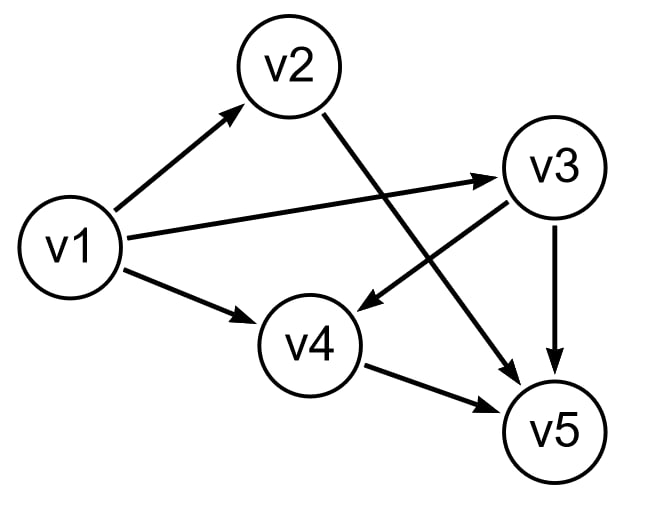
\includegraphics[width=0.3\linewidth]{counterexamplegraph.jpg}
      \end{figure}
    This is an example of a graph which will not give the correct answer.
    The longest path would be 4, from v1, v3, v4, v5.
    With the algorithm, we will take the path v1, v2, v5.
    This is because the algorithm takes into account the very first neighbour node only.
    Thus, it ignores all other paths and continues executing the algorithm.
    In such a case, v3 actually provides the longest path, but it ignores it as it starts processing v2 immediately. 
    \item
    \lstset{caption={DFS DP Longest Path}}
    \lstset{label={lst:alg1}, numbers=left}
    \begin{lstlisting}[style = Python]
        def longest_path(src: int, n: int, adj_list: list[list]) -> int:
            dp = [1] * (n + 1) 
            # to keep track of nodes seen to avoid double counting
            visited = set()
            
            def dfs(node):
                visited.add(node)
                for neighbour in adj_list[node]:
                    # find the longest path of neighbours first
                    if neighbour not in visited:
                        dfs(neighbour)
                    # recurrence that the neighbour's optimal longest path
                    # has been resolved already
                    dp[node] = max(dp[node], dp[neighbour] + 1)
            
            for i in range(1, n + 1):
                if i not in visited:
                    dfs(i)
            
            return dp[src]        
  \end{lstlisting}
    We can perform DFS with DP and a visited set to find the longest path in the DAG. 
    To find the longest path between two nodes in a DAG,
    we can first find the longest path between a node and its neighbour.
    Through this subproblem, we can store the result in a dp array.
    We can then work on bigger problems, iterating the neighbours
    and trying to find the subproblem which gives us the maximum length.
    Due to the iteration and dfs nature, we are guaranteed to solve our neighbour's subproblems first due to the lack of cycles. \\\\
    
    Recurrence: We can form a recurrence relation based on the following: \\
    \[
       dp[node] = max(dp[node], dp[neighbour] + 1)
    \]
    A brief explanation would be that since a node has many neighbours,
    it has either found a longest path already, or one of its neighbours can be built off and provide an even longer path. \\
    
    Runtime: $O(n^2)$ due to iterating n nodes, 
    and potentially performing dfs on each node, where dfs iterates the adjacency list. 
    There can potentially be up to n-1 neighbours in the adjacency list, which is bounded by n. Hence quadratic time complexity.
\end{enumerate}

\end{document}
